\documentclass[aspectratio=1610]{beamer}
\hypersetup{
        unicode=true,
        linkcolor=blue,
        anchorcolor=blue,
        citecolor=green,
        filecolor=black,
        urlcolor=blue
    }

%%%%% PACKAGES HERE
%% \usepackage{}
\usepackage{amsmath}
\usepackage{amssymb}
\usepackage{listings}


\usepackage[style=authortitle,backend=biber]{biblatex}
\addbibresource{references.bib}

%%%%%%%%%%%%%%%%%%%%%%%%%%%%%%%%%%%
%% DO NOT CHANGE

\usetheme{default}
\useinnertheme{circles}
\useoutertheme{infolines}
\usefonttheme{serif}

\usepackage{etoolbox}

%% T for navigation symbols
%%\setbeamertemplate{navigation symbols}{}

%% T for header
%% \setbeamertemplate{headline}{%
%%   \leavevmode%
%%   \ifdefempty{\insertsubsectionhead}{
%%     \begin{beamercolorbox}[wd=0.99\paperwidth,ht=2.25ex,dp=1ex,center]{section in head/foot}%
%%       % \hbox to .5\paperwidth{\hfil\insertsectionhead\hfil}
%%       \insertsectionhead
%%     \end{beamercolorbox}%
%%   }{
%%     \begin{beamercolorbox}[wd=.44\paperwidth,ht=2.25ex,dp=1ex,right]{section in head/foot}%
%%       % \hbox to .5\paperwidth{\hfil\insertsectionhead\hfil}
%%       \insertsectionhead
%%     \end{beamercolorbox}%
%%     \begin{beamercolorbox}[wd=.1\paperwidth,ht=2.25ex,dp=1ex,center]{section in head/foot}%
%%       % \hbox to .5\paperwidth{\hfil\insertsectionhead\hfil}
%%       -
%%     \end{beamercolorbox}%
%%     \begin{beamercolorbox}[wd=.44\paperwidth,ht=2.25ex,dp=1ex,left]{subsection in head/foot}%
%%       % \hbox to .5\paperwidth{\hfil\insertsubsectionhead\hfil}
%%       \insertsubsectionhead
%%     \end{beamercolorbox}
%%   }%
%% }

%% T for frame title
\setbeamertemplate{frametitle}{%
  \usebeamerfont{frametitle}\insertframetitle\strut%
  \vskip-0\baselineskip%
  \leaders\vrule width .95\paperwidth\vskip1pt%
  \vskip0pt%
  \nointerlineskip
}

%% T for footer
\setbeamercolor{footlinecolor}{fg=cyan,bg=green}
\setbeamercolor{author in head/foot}{fg=blue}

\setbeamertemplate{footline}{%
  \leavevmode%
  \hbox{%
  \begin{beamercolorbox}[wd=.26\paperwidth,ht=2.25ex,dp=1ex,left]{author in head/foot}%
    \hspace*{2ex}\usebeamerfont{author in head/foot} Mattia Bruno Stellacci
  \end{beamercolorbox}%
  \begin{beamercolorbox}[wd=.50\paperwidth,ht=2.25ex,dp=1ex,center]{author in head/foot}%
    \usebeamerfont{title in head/foot}A Visual Exploration of Manifold Learning for Images
  \end{beamercolorbox}%
  \begin{beamercolorbox}[wd=.24\paperwidth,ht=2.25ex,dp=1ex,right]{date in head/foot}%
    \usebeamerfont{date in head/foot}
    \insertshortdate{}\hspace*{1em}  % date
    \insertframenumber/\inserttotalframenumber\hspace*{2ex}
  \end{beamercolorbox}}%
  \vskip0pt%
}
%%%%%%%%%%%%%%%%%%%%%%%%%%%%%%%%%%%%%%%%%%%%%%%%

%% Start from here.
\title{Project Report:\\
A Visual Exploration of Manifold Learning for Images}
\author{Mattia Bruno Stellacci}
\date\today

\begin{document}

\begin{frame}[plain]
  \titlepage
  % // Title page \footcite{nasy_beamer_2022}
\end{frame}


\begin{frame}{Outline}
  \tableofcontents

  \end{frame}
  % // This frame is the outline page which contains the full outline.


% \begin{frame}
%   \tableofcontents[currentsection, subsectionstyle=show/show/hide]

%   % // This frame is the outline page for frame Introduction
% \end{frame}

\section{Introduction}

\subsection {Motivation}
\begin{frame}
  \frametitle{Motivation}
  \begin{itemize}
    \item Create a system to facilitate understanding dimensionality reduction for images
    \item{\textit{Why dimensionality Reduction?}}   
    \item{\textit{Why images?}} % Prime example of high-extrinsic dimension yet easy to grasp.   
    \item Allow the user to visualize and manipulate raw data and lower-dimensional embeddings
    \item Allow users to compare different dimensionality reduction techniques  
  \end{itemize}
\end{frame}


\subsection {Goals}
\begin{frame}
  \frametitle{Goals}

  \begin{itemize}
      \item Build a powerful, modern Visual Analytics platform in the browser
      \item Harness a \texttt{WebAssembly} port of \texttt{OpenCV} to incorporate image manipulation in the browser
      \item Incorporate multiple dimensionality reduction/manifold learning techniques to allow users to compare them conveniently. 
      \item Create visual support for some of the notable properties of lower-dimensional embeddings: Clustering of similar instances,separability, Variance, Compactness. 
  \end{itemize}

\end{frame}

\subsection {Target Audience/Intended Users}
\begin{frame}
  \frametitle{Intended Users}

  \begin{itemize}
      \item \textbf{Students} %looking to understand dimensionality reduction/manifold learning
      \item \textbf{Machine learning engineers/Data scientists}  % determining suited dimensionality reductions techniques for their application
  \end{itemize}

\end{frame}

\subsection {Related Work}
\begin{frame}
  \frametitle{Related Work}
  \begin{itemize}
    \item Dimensionality Reduction extremely common for Data Visualization: \begin{itemize}
      \item Many publications in the 00's focus on/describe the techniques themselves.
      \item 2000: 'A global geometric framework for nonlinear dimensionality reduction'
      \item 2010 Survey: "Data Visualization: Manifold Learning for Visualizing and Analyzing High-Dimensional Data" 
      \item Later papers make use of this technique to visualize their data, less focussed on the techniques \textit{per se}

    \end{itemize}
    \item Big Data: \textit{Curse of Dimensionality}
    \item Machine Learning: New found interest in dimensionality reduction, the Manifold hypothesis:\begin{itemize}
      \item Word Embeddings (word2vec)
      \item Generative models (VAE)
    \end{itemize}

    \item Couldn't find a work on a visual analytics system that combines dimensionality reduction/manifold learning for images with automatic image processing
  \end{itemize}

\end{frame}


\section {Implementation}
\begin{frame}
    \begin{centering}
      \huge{Implementation}
    \end{centering}
\end{frame}

\begin{frame}
  \hspace{4em}
  \frametitle{Reminder: Vision/Mockup}
    \begin{centering}
      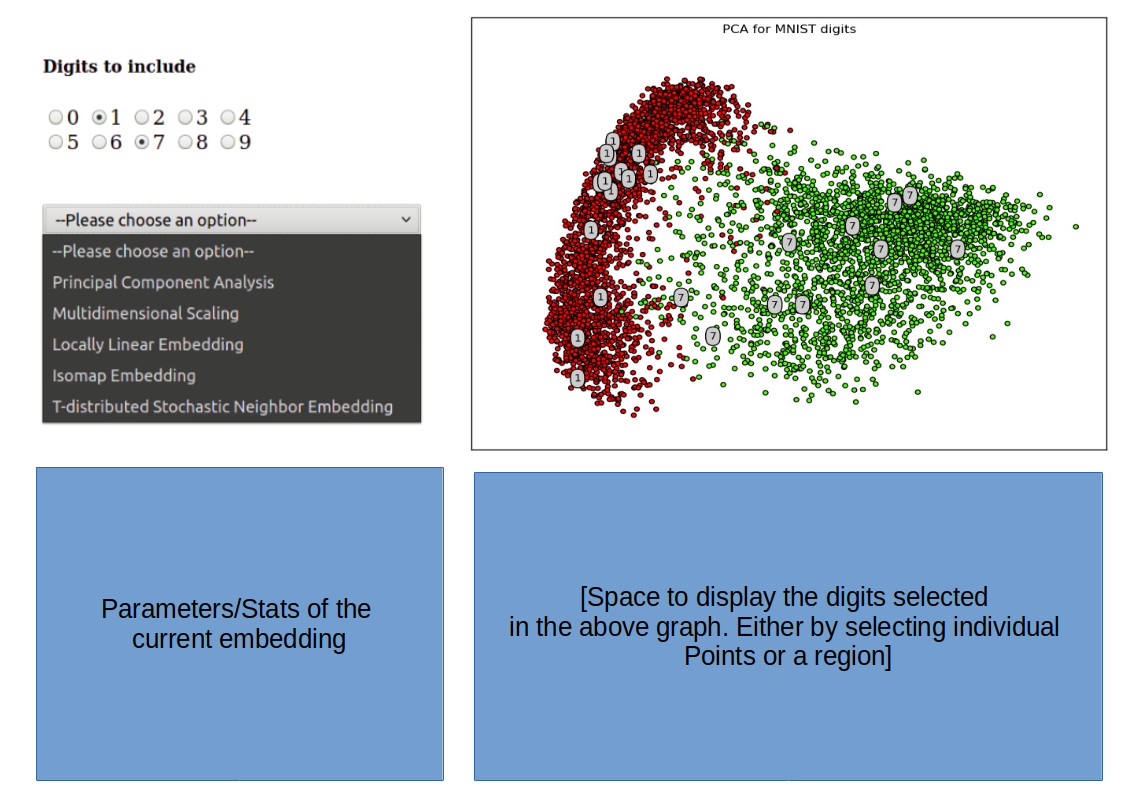
\includegraphics[height=.5\textwidth]{fig/mockup_va.png}
    \end{centering}

\end{frame}

\subsection {Tech stack}
\begin{frame}
  \frametitle{Technologies I chose:}

  \begin{itemize}
      \item \textbf{Dataset:} MNIST Handwritten Digits %looking to understand dimensionality reduction/manifold learning
      \item \textbf{Frontend:} \texttt{ReactJS} %looking to understand dimensionality reduction/manifold learning
      \item \textbf{Charting Library:} \texttt{react-vis} {\tiny (RIP)}
      \item \textbf{Backend/Embedding:}  \begin{itemize}
        \item Python/\texttt{bottle}
        \item \texttt{scikit-learn}  % determining suited dimensionality reductions techniques for their application
      \end{itemize}
      \item \textbf{Image Processing:} \texttt{OpenCV}
  \end{itemize}

\end{frame}

\subsection {Dimensionality Reduction techniques}
\begin{frame}
  \frametitle{Dimensionality Reduction techniques}

  \large{\underline{Dimensionality reduction techniques I included:}}
  \begin{itemize}
    \item \textbf{Principal Component Analysis} 
    \item \textbf{Isomap embedding}       
    \item \textbf{Locally Linear Embedding}    
  \end{itemize}
  \large{\underline{Didn't make the cut:}}
  \begin{itemize}
    \item \textbf{TSNE} 
    \item \textbf{MDS}       
    \item \textbf{Variational Autoencoder}    
  \end{itemize}
\end{frame}

\section {Insights}
\begin{frame}
  \frametitle{Insights I gained/Challenges I encountered:}
  \begin{itemize}
    \item \textbf{Diversity:} One size does not fit all.
    \item \textbf{Explainability} What do the results mean?
    \item \textbf{Comparability} Random Sampling from huge Dataset might not be the best idea.
    \item \textbf{Interpretebality:} Sampling and Inverse transform. 
    \item \textbf{Specificity}: Focus on a single case.
    \item \underline{\textbf{Bidirectionality:} Harness the true power of interactivity and aggregation}      
  \end{itemize}
\end{frame}

\section {Demo}
\begin{frame}
    \begin{centering}
      \huge{Demo}
    \end{centering}
\end{frame}

\section {Conclusion}
\begin{frame}
    \begin{centering}
      \huge{Conclusion}
    \end{centering}
\end{frame}

\end{document}

% \begin{frame}
%   \tableofcontents[currentsection, subsectionstyle=show/show/hide]
% \end{frame}